%
% 3dimagetemplate.tex
%
% (c) 2018 Prof Dr Andreas Müller, Hochschule Rapperswil
%
\documentclass[tikz,12pt]{standalone}
\usepackage{times}
\usepackage{amsmath}
\usepackage{txfonts}
\usepackage[utf8]{inputenc}
\usepackage{graphics}
\usetikzlibrary{arrows,intersections,math}
\usepackage{ifthen}
\begin{document}

\newboolean{showgrid}
\setboolean{showgrid}{false}
\def\breite{7}
\def\hoehe{4}

\begin{tikzpicture}[>=latex,thick,scale=1.07]

% Povray Bild
\node at (0,0) {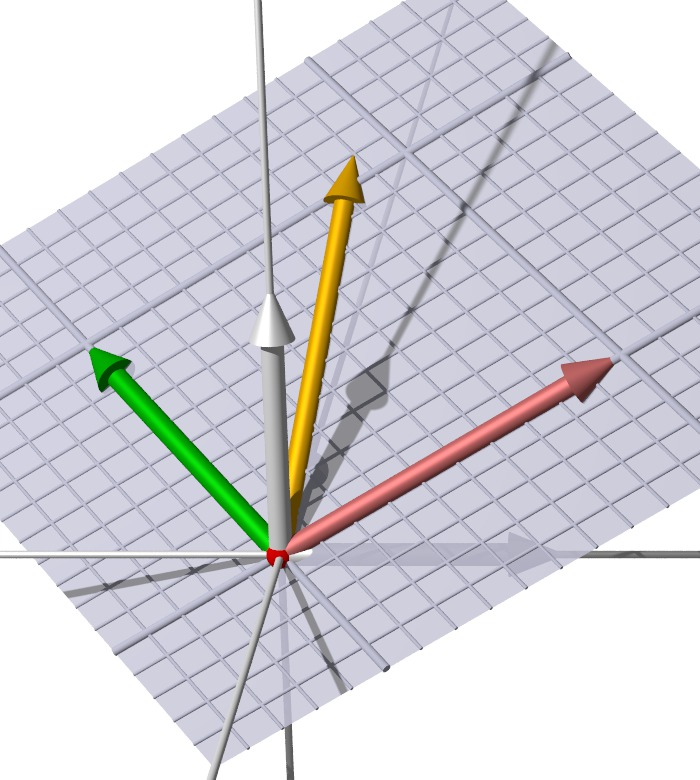
\includegraphics[width=5.1cm]{basis.jpg}};
\node at (-5,0) {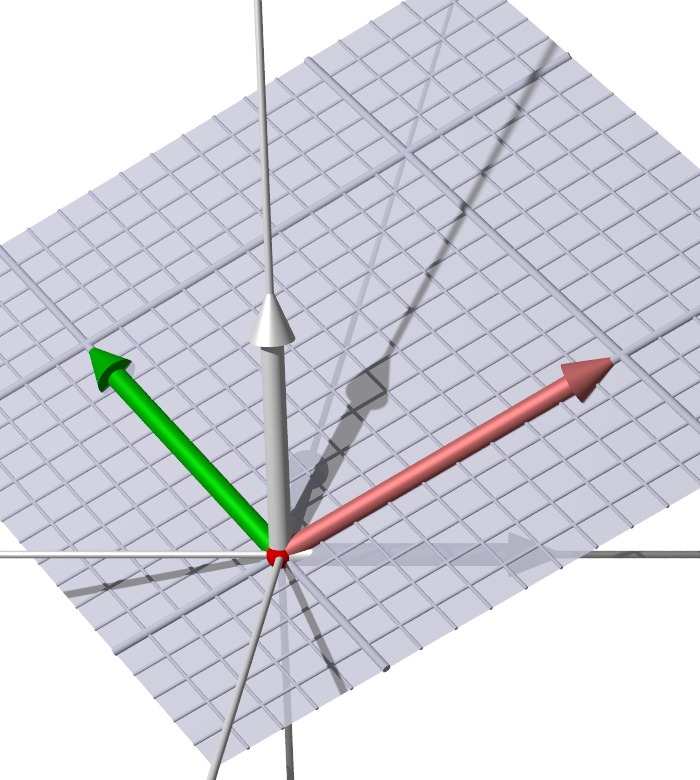
\includegraphics[width=5.1cm]{basis2.jpg}};
\node at (5,0) {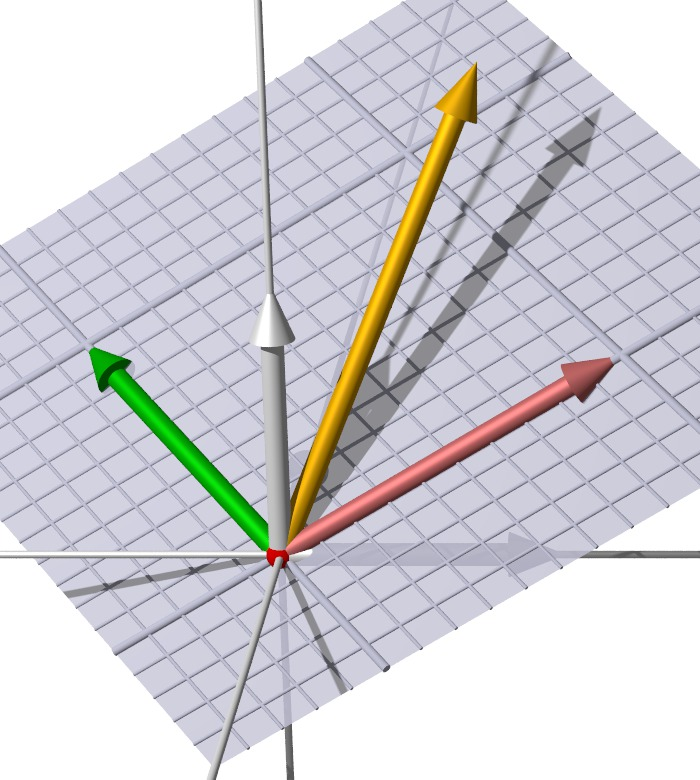
\includegraphics[width=5.1cm]{basis3.jpg}};

% Gitter
\ifthenelse{\boolean{showgrid}}{
\draw[step=0.1,line width=0.1pt] (-\breite,-\hoehe) grid (\breite, \hoehe);
\draw[step=0.5,line width=0.4pt] (-\breite,-\hoehe) grid (\breite, \hoehe);
\draw                            (-\breite,-\hoehe) grid (\breite, \hoehe);
\fill (0,0) circle[radius=0.05];
}{}

% lettering
\node at (-4,-2) {a)};
\node at ( 1,-2) {b)};
\node at ( 6,-2) {c)};

\end{tikzpicture}

\end{document}

